\section{Evaluation}\label{sec:eval}

We evaluate \( \tool \) based on the following four research questions:
\begin{itemize}
  \item RQ2) \textbf{Effectiveness} Is \( \tool \) effective to extract syntax and
    semantics of existing ECMAScript specifications?
  \item RQ1) \textbf{Correctness} Does \( \tool \) correctly extract JavaScript syntax
    and semantics from ECMAScript 2020 speicification?
  \item RQ3) \textbf{Adaptability} Does \( \tool \) deal with future proposed features?
  \item RQ4) \textbf{Specification Error Detection} What specification errors
    are detected by \( \tool \)?
\end{itemize}

\subsection{Effectiveness}

\begin{figure}[t]
  \[
    \begin{array}{c|r|r|r|r|r?r}
      \hline
      \textbf{version}
      & \multicolumn{1}{c|}{\textbf{2016}}
      & \multicolumn{1}{c|}{\textbf{2017}}
      & \multicolumn{1}{c|}{\textbf{2018}}
      & \multicolumn{1}{c|}{\textbf{2019}}
      & \multicolumn{1}{c?}{\textbf{2020}}
      & \multicolumn{1}{c}{\textbf{avg.}}\\\hline
      \text{\# lexical prod.}
      & \text{78}
      & \text{78}
      & \text{78}
      & \text{81}
      & \text{81}
      & \text{79.2}\\\hline
      \text{\# syntactic prod.}
      & \text{157}
      & \text{167}
      & \text{167}
      & \text{174}
      & \text{175}
      & \text{168}\\\hline
    \end{array}
  \]
  \[
    \begin{array}{c|r|r|r|r?r}
      \hline
      \textbf{old version}
      & \multicolumn{1}{c|}{\textbf{2016}}
      & \multicolumn{1}{c|}{\textbf{2017}}
      & \multicolumn{1}{c|}{\textbf{2018}}
      & \multicolumn{1}{c?}{\textbf{2019}}
      & \multirow{2}{*}{\textbf{avg.}}\\\cline{1-5}
      \textbf{new version}
      & \multicolumn{1}{c|}{\textbf{2017}}
      & \multicolumn{1}{c|}{\textbf{2018}}
      & \multicolumn{1}{c|}{\textbf{2019}}
      & \multicolumn{1}{c?}{\textbf{2020}}
      & \\\hline
      \Delta \; \text{\# lexical prod.}
      & \text{3}
      & \text{5}
      & \text{6}
      & \text{0}
      & \text{4.7}\\\hline
      \Delta \; \text{\# syntactic prod.}
      & \text{140}
      & \text{15}
      & \text{8}
      & \text{2}
      & \text{55}\\\hline
    \end{array}
  \]
  \caption{The number of productions for lexical and
  syntactic grammars in ECMAScript specifications.}
  \label{fig:syntax-all-version}
\end{figure}

\begin{figure}[t]
  \centering
  \begin{subfigure}{0.23\textwidth}
    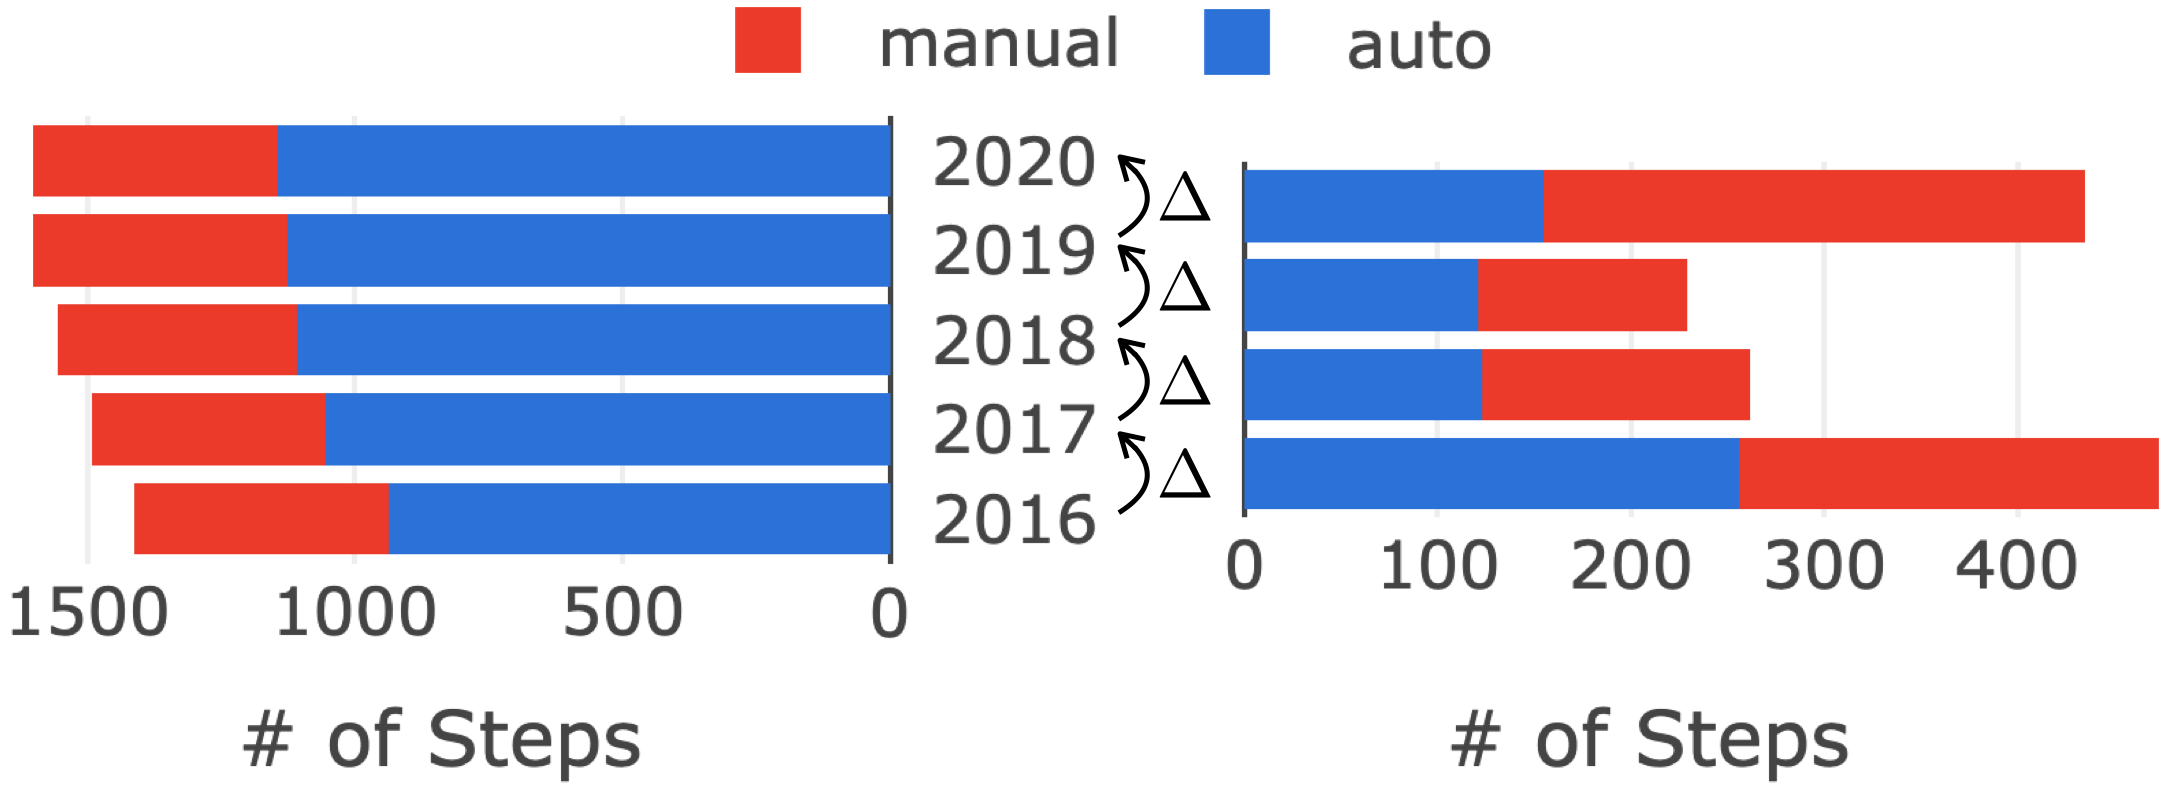
\includegraphics[width=\textwidth]{img/all-version-sem.png}
    \caption{Evaluation results for each version}
    \label{fig:semantics-all-version}
  \end{subfigure}
  \hfill
  \begin{subfigure}{0.20\textwidth}
    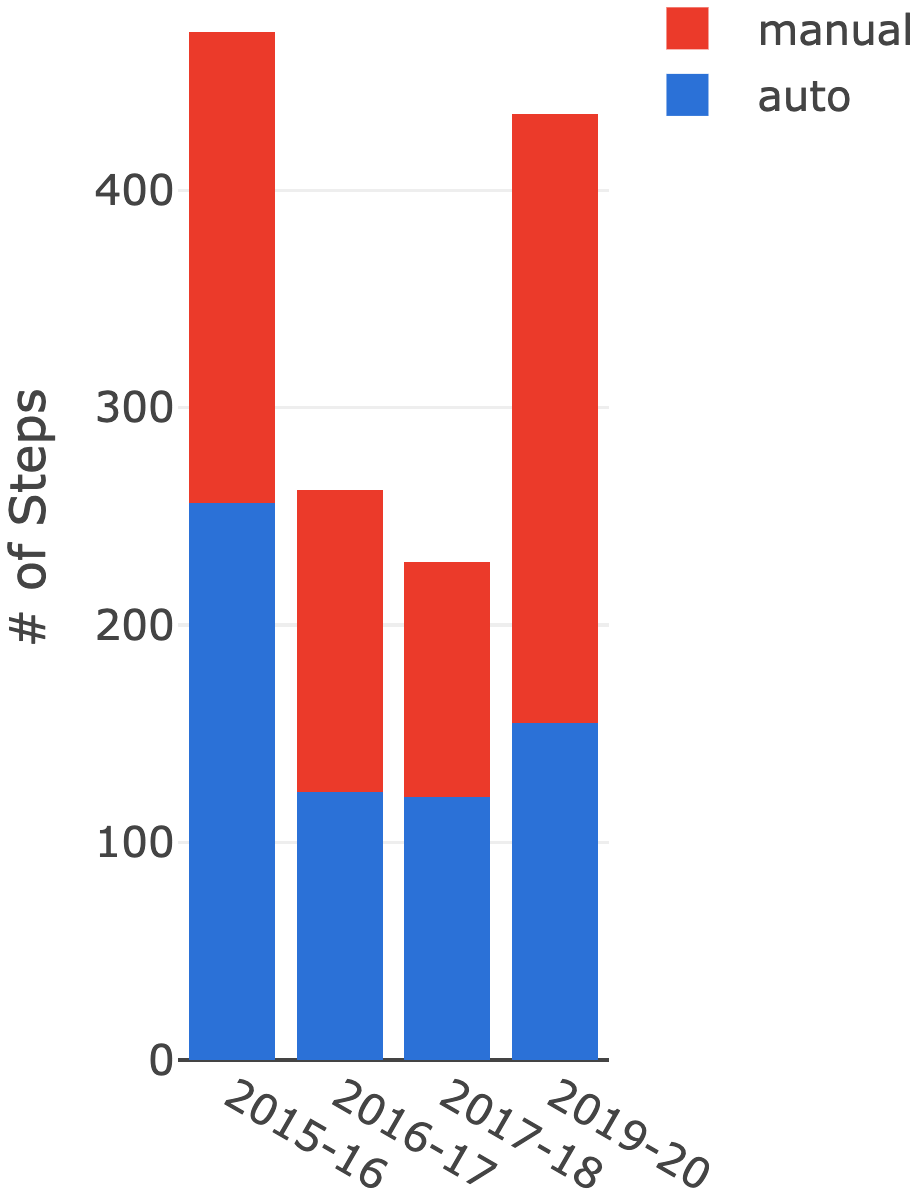
\includegraphics[width=\textwidth]{img/all-version-sem-delta.png}
    \caption{Evaluation results for each difference of adjacent versions}
    \label{fig:semantics-all-version-delta}
  \end{subfigure}
  \caption{The result of the parser generator and the algorithm compiler for
  ECMAScript specifications.}
  \label{fig:all-version}
\end{figure}

We discuss the effectiveness of \( \tool \) by applying it into existing ECMAScript specifications.
The evaluation focuses on how many productions and abstract algorithms are covered by
our tool 1) in each version, and 2) in each difference between adjacent versions.
Figure~\ref{fig:all-version} shows the result of \( \tool \) from ECMAScript 2016
to 2020. While ECMAScript 5.1 is the first version that officially supports
the specification in HTML. However, two oldest versions ECMAScript 5.1 and 2015 are written
in quite different styles with recent versions including HTML tags used in abstract algorithms.
Thus, we evaluate only five recent versions from ECMAScript 2016 to 2020.

First, we evaluate that the \textsf{Parser Generator} in \( \tool \) successfully generate
parsers from all target versions of ECMAScript specifications. As described in
Figure~\ref{fig:syntax-all-version}, lexical and syntactic grammars
have \inred{XX} and \inred{XXX} productions in average, respectively.
Moreover, JavaScript syntax are annually updated of \inred{X} productions for lexical grammars
and \inred{XX} productions for syntactic grammars in average.

Figure~\ref{fig:all-version} shows the evaluation results for semantics.
The \textsf{Algorithm Compiler} with the compile rules described in Section~\ref{sec:impl}
has \inred{XX\%} success rates for existing specifications in average. Moreover,
\( \tool \) are also effective to update existing semantics
because \inred{XX\%} of changed or newly defined algorithms are automatically
compiled into \( \ires \) functions. Thus, we believe that \( \tool \) effectively
reduce the effort to extract syntax and semantics of JavaScript
not only when developing them from the scratch, but also updating existing syntax and semantics.

\subsection{Correctness}

\begin{table}
  \centering
  \begin{tabular}{lr}\toprule
    \belowrulesepcolor{gainsboro}
    \rowcolor{gainsboro} \textbf{All tests262 Tests} & \textbf{36,794}\\
    \aboverulesepcolor{gainsboro}\midrule
    Annexes/Internationalisation & 1,774\\\hdashline
    In-progress features & 5,803\\\midrule
    \belowrulesepcolor{gainsboro}
    \rowcolor{gainsboro} \textbf{ECMAScript 2020 Tests} & \textbf{29,217}\\
    \aboverulesepcolor{gainsboro}\midrule
    Non-strict codes & 1,136\\\hdashline
    Modules & 918 \\\hdashline
    Negative tests & 2,280\\\hdashline
    \code{Math}, \code{Date}, \code{RegExp}, and \code{JSON} & \inred{XXXX}\\\midrule
    \belowrulesepcolor{gainsboro}
    \rowcolor{gainsboro} \textbf{Applicable Tests} & \textbf{\inred{XXXXX}}\\
    \aboverulesepcolor{gainsboro}\midrule
    Not-yet modeled & \inred{XXXX} \\\hdashline
    Passed tests & \inred{XXXX} \\\hdashline
    Failed tests & \inred{XXXX} \\\bottomrule
  \end{tabular}
  \caption{The results of tests in the test262 for ECMAScript 2020.}
  \label{table:test262}
\end{table}

To evaluate that \( \tool \) correctly extracts semantics, we develop the JavaScript
interpreter based on the extracted syntax and semantics from ECMAScript 2020.
Among \inred{XXXX} algorithms in ECMAScript 2020, \inred{XXX} algorithms
are related to the not-supported language features. And \inred{XXXX} algorithms
are automatically compiled into \( \ires \) functions via the \textsf{Algorithm Compiler}.
Among remaining \inred{XXX} algorithms, we select \inred{XX} algorithms
essential parts of overall semantics and manually implement corresponding \( \ires \)
functions. As described in Section~\ref{sec:impl}, we also
carefully implement \textsf{Global Setting}.

We test our JavaScript interpreter based on test262, the conformance test suite
that is officially provided by the committee TC39. However, the current version of
test262 also provides tests for other extensions or in-progress features.
Thus, we exclude them to focus on only the semantics of ECMAScript 2020.
Figure~\ref{table:test262} describes how to break down tests and the test results of extracted
semantics. We use test262 written in \inred{August 6, 2019}. In that version,
test262 consists of 36,794 tests and we first exclude \inred{XXXX} tests
for extensions and in-progres features. We also remove \inred{XXXX} tests for
not-supported features; non-strict codes, intricate built-in objects, and modules.
Finally, we tested \inred{XXXXX} applicable tests with our JavaScript interpreter.
Among them, \inred{XXXXX} tests are successfully passed and all other tests are
not passed just because of not yet modeled abstract algorithms. It means that
all semantics extracted from \( \tool \) are perfectly correct.

% TODO if some tests are failed, categorize them and explain why they are failed.

\subsection{Adaptability}

We also check that \( \tool \) deals with future language features for adaptability.
ECMAScript specifications are managed as open-sources and proposals of in-progress language
features by following the TC39 process. Such proposals are tracked in the separated repository~\cite{proposals}
and thare are six different stages for them; Stage from 0 to 3, and finished or inactive proposals.
Each proposal starts with Stage 0 and is promoted into Stage 3 through Stage 1 and 2.
The committee (TC39) regularly examins the Stage 3 proposals to decide their next stages.
If the proposals are confirmed, the committee changes their stages into finished
and integrate them into the next version of ECMAScript specification.
Otherwise, the committee changes them into inactive. Our tool \( \tool \) is also applicable
into not yet finished proposals and we advance a case study for a Stage 3 proposal.

The optional chain syntax (\( \code{?.} \)) is one of Stage 3 proposals that removes the
boilerplate codes; \( \code{x \&\& x.p} \). The code first checks that the value of
the variable \( \code{x} \) is not \( \code{undefined} \) and then access its
property \( \code{p} \). With the optional chain syntax, we could redece the code size
by implementing as \( \code{x?.p} \). We apply this proposal into ECMAScript 2020 specification
and evaluate \( \tool \) to extract the semantics from the extended specification.
For the extended speicification, the \textsf{Parser Generator} successfully handle
three updated lexical productions and three updated syntactic productions.
For semantics, there 22 updated abstract algorithms. At the first attempt,
the \textsf{Algorithm Compiler} suceedes to compile only 10 algorithms.
However, we notice that several algorithm steps have diffrent styles with
the existing ECMAScript specifications. Thus, we revise them into the original
writing styles and report the revision into the GitHub repository of the proposal.
The authors of this proposal approved and accepted our pull requests.
After revisions, 21 of 22 algorithms are successfully compiled and we manually
compile only one algorithm. In the test262, there are 33 tests related to the optional chain
syntax and six tests of them are semantics tests. The semantics extracted with
the optional chain proposal successfully pass all the six semantics tests.
This case study shows the adaptability of \( \tool \) for future language features
and also \( \tool \) might be possible to be used as a specification writing guidance.

\subsection{Specification Error Detection}

We found three specification errors in ECMAScript 2020 via \( \tool \).
We fixed them and sent pull requests into the official GitHub repository of
ECMAScript specification~\cite{es2020}. They were all confirmed by TC39
and will be fixed in the next release.

First, we found that \textbf{VarScopedDeclarations} syntax-directed algorithms of
specific cases of \textit{IterationStatement} are ambigious.
The \textbf{VarScopedDeclarations} algorithm is used to initially define
the variable declarations before entering speicific scopes.
However, the following iteration syntax has two different
\textbf{VarScopedDeclarations} algorithms:
\[
  \code{for await (} \; \textit{LeftHandSideExpression} \; \code{of} \;
\textit{AssignmentExpression} \; \code{)} \; \textit{Statement}
\]
The \textsf{Spec Extractor} of \( \tool \) detects its duplicated
semantics during automatically extracting abstract algorithms into JSON files.

For the \textbf{ExpectedArgumentCount} algorithm, we found that
there are missing cases for some syntax. This algorithm counts the number of
expected arugments of a specific parameters. However, it does not cover all
the cases. For example, if there exists only one formal parameter,
the ECMAScript 2020 specification does not provide any semantics.
We detect this error during evaluations of test262 tests under
the extracted semantics via \( \tool \). It throws an error that there
is no \textbf{ExpectedArgumentCount} algorithm for specific tests.

Moreover, we found an error in \textsf{Ecmarkup}, a toolchain used to
specify ECMAScript and beautify a raw speicification HTML file
into a more visible HTML file. At the first time, we though that
we found a missing case for the \textbf{IsFunctionDefinition}
algorithm of unnamed function expressions. However, in the
raw specification HTML file, there are no missing cases. We investigate
why it happens and realize that \textsf{Ecmarkup} itself has
a bug to silently remove the {\small opt} subscript in \( \code{collapsed} \)
syntax mode. It is already discovered bug but our tool found this bug
in a mechanical way.
